%\section{Problem Overview}\label{sec: background}
%formalize the task of identifying vulnerable libraries and introduce the scalability limitation of existing ranking approaches.
% To address the scalability limitation, we model this task as a generation task based on the results of an empirical study and then investigate the challenges of generating the names of affected packages.


\begin{table*}[t]
    \centering
    \caption{An Empirical Study on ChatGPT's Incorrect Response in Maven (Java ecosystem)}
    \label{tab: fault case study}
\scriptsize
\begin{threeparttable}
\begin{tabular}{p{2cm}p{1.8cm}p{4.3cm}p{4.3cm}}
\toprule
\textbf{Error Reason}                                            & Example (w/ link)                             & ChatGPT's Output                                                   & Ground Truth (Affected Packages)                                                         \\
\midrule
\multirow{2}{*}{\makecell[l]{\textbf{Type 1: Incorrect}\\ \textbf{but exist (23\% of}\\ \textbf{ all errors)}}} & \href{https://github.com/advisories/GHSA-9qhq-j4xm-cw48}{CVE-2015-3158}                     & org.\textcolor{Blue}{picketlink:picketlink}                                    & org.\textcolor{Blue}{picketlink:picketlink-tomcat}-common                                     \\
&&  \multicolumn{2}{l}{\textit{Description:} ``The invokeNextValve function in \textit{identity/federation/bindings/\textcolor{Blue}{tomcat}/idp/AbstractIDPValve.java}}                             \\
&& \multicolumn{2}{l}{in \textcolor{Blue}{PicketLink} before 2.7.1.Final does not properly check role based authorization, which allows remote} \\
&& \multicolumn{2}{l}{authenticated users to gain access to restricted application resources via a (1) direct request $\dots$'' } \\
\midrule
\multirow{8}{*}{\makecell[l]{\textbf{Type 2: Non-Exist,}\\ \textbf{Partially correct}\\ \textbf{(58\% of all errors)}}}                                          & \href{https://github.com/advisories/GHSA-wv88-pf73-x22p}{CVE-2011-2730}                     & org.\textcolor{Blue}{springframework}:\textcolor{Red}{spring-framework}                                    & org.\textcolor{Blue}{springframework}:\textcolor{Blue}{spring-core}                                      \\
&&  \multicolumn{2}{l}{\textit{Description:} ``VMware \textcolor{Blue}{SpringSource Spring Framework} before 2.5.6.SEC03, 2.5.7.SR023, and 3.x before  }                                                                                                                                                                                \\
&& \multicolumn{2}{l}{ 3.0.6, when a container supports Expression Language (EL), evaluates EL expressions in tags twice which } \\
& & \multicolumn{2}{l}{allows remote attackers to obtain sensitive information. $\dots$''}                                                                                                                                                                                \\
\cmidrule(lr){3-4}
% , and ChatGPT mistakes token ``\textcolor{BrickRed}{framework}'' in its artifact ID.
  & \href{https://github.com/advisories/GHSA-264w-xrr7-6qqg}{CVE-2020-2167}                       & \textcolor{Red}{org.jenkins-ci.plugins}:\textcolor{Blue}{openshift-pipeline}                    & \textcolor{Blue}{com.openshift.jenkins}:\textcolor{Blue}{openshift-pipeline}                       \\
&&\multicolumn{2}{l}{\textit{Description:} ``\textcolor{Blue}{OpenShift Pipeline Plugin} 1.0.56 and earlier does not configure its YAML parser to prevent} \\
&&\multicolumn{2}{l}{
the instantiation of arbitrary types. This results in a remote code execution (RCE) vulnerability exploitable}                                                                                                                                                                      \\
&& \multicolumn{2}{l}{  by users able to provide YAML input files to OpenShift Pipeline Plugin’s build step. $\dots$''}                                                                                                                                                                      \\
 % without the group id, so ChatGPT uses a widely used one ``\textcolor{BrickRed}{org.jenkins-ci.plugins}''.
\midrule
% \textbf{More/Fewer Tokens}                      & 28                        & \href{https://github.com/advisories/GHSA-3v63-f83x-37x4}{CVE-2015-1830}                       & org.apache.activemq:activemq                                 & org.apache.activemq:activemq-client                            \\
% \multicolumn{5}{l}{\textit{Description:} ``Directory traversal vulnerability $\dots$ in \textcolor{ForestGreen}{Apache ActiveMQ} 5.x before 5.11.2 $\dots$'', and ChatGPT lacks the token ``\textcolor{ForestGreen}{client}''.}                                                                                                                                                                                      \\
% \midrule
\multirow{4}{*}{\makecell[l]{\textbf{Type 3: Non-Exist,}\\ \textbf{Completely incorrect}\\ \textbf{(19\% of all errors)}}}&                      \href{https://github.com/advisories/GHSA-jpj4-5xwp-cv23}{CVE-2020-11974}                      & \textcolor{Red}{mysql:mysql-connector-java}                                   & \textcolor{Blue}{org.apache.dolphinscheduler:dolphinscheduler}                   \\
&& \multicolumn{2}{l}{\textit{Description:} ``In \textcolor{Blue}{DolphinScheduler} 1.2.0 and 1.2.1, with \textcolor{Red}{mysql connector} a remote code execution vulnerab}\\
&& \multicolumn{2}{l}{-ility
exists when choosing mysql as database.''}                          \\
\cmidrule(lr){3-4}
% , and ChatGPT incorrectly captures ``\textcolor{BrickRed}{mysql}''.
&          \href{https://github.com/advisories/GHSA-fxp8-7h5w-h235}{CVE-2019-13234}                      & \textcolor{Red}{N/A}                                                                  & \textcolor{Blue}{org.opencms:opencms-core}                                       \\
&&\multicolumn{2}{l}{\textit{Description:} ``In the Alkacon \textcolor{Blue}{OpenCms} Apollo Template 10.5.4 and 10.5.5 there is XSS in the search engine.''}  \\
% , and ChatGPT repeats the unstructured description.
\bottomrule
\end{tabular}
% \begin{tablenotes}
%     \item A Java package name consists of two parts, [group id]:[artifact id]
% \end{tablenotes}
\end{threeparttable}
\vspace{-0.3cm}
\end{table*}



%\subsection{Task Formalization}~\label{sec: formal}
%\noindent \textbf{Target:}


% and the developer description may not explicitly differentiate between them\xueqing{provide a concrete example}. 

%The following is backup
% Given a natural language description of the vulnerability associated with a software package (e.g., Figure~\ref{fig: case}), the goal is to identify the software package that the description refers to. For example, the description in Figure~\ref{fig: case} refers to the Java package \CodeIn{org.jenkins-ci.plugins:mailcommander}. The referred package must be within the existing packages of the ecosystem (e.g., Table~\ref{tab: dataset info}). The ground truth package name is verified by expert maintainers from the GitHub advisory database~\cite{githubReview}. From Figure~\ref{fig: case} we observe that the identification of the package name is a non-trivial problem that goes beyond token-level matching. The challenges of this NLP task lie in the following folds: first, a part of the target package name is missing in the description, which requires domain knowledge for bridging this gap\xueqing{provide a concrete example}; second, some package names are similar, so it is easy to confuse between them, e.g., \CodeIn{org.jenkins-ci.plugins} and \CodeIn{io.jenkins.plugins} are two most common group IDs in Java, and the developer description may not explicitly differentiate between them\xueqing{provide a concrete example}. 


%The mapping results are defined as subsets of $\mathcal{L}$ as one vulnerability can affect more than one package: $\forall v \in \mathcal{V}, \mathcal{F}(v) \subseteq \mathcal{L}$.

% \noindent \textbf{Labelled Dataset:}

% The dataset $\mathcal{D}$ of this task includes $(\mathcal{V_D}, \mathcal{L_D}, \mathcal{F_D})$ where $\mathcal{V_D}$ is a set of collected vulnerabilities, $\mathcal{F_D}$ is the labels (affected packages) of these vulnerabilities, and $\mathcal{L_D}$ is naturally defined as $\mathcal{F_D}(V_D)$.

% The target of existing approaches is to learn the correlation from a given dataset $\mathcal{F^{'}} \sim \mathcal{F_D}$.



\section{Existing Work on Vulnerable Package Identification\label{sec: scale}}

This section summarizes existing work on affected package identification and analyze the scalability challenge. 

\noindent \textbf{Formal Definition of Affected Package Identification}. Given a security vulnerability (CVE) submitted to a software ecosystem (e.g., GitHub Advisory), the goal of affected package identification is to link the description $q$ of the CVE to an existing software package name $p$ (e.g., a Maven or PyPi package) that is affected by the CVE. An example of the linked package can be found in Figure~\ref{fig: case}, where the description mentions the affected package \CodeIn{org.jenkins-ci.plugins:mailcommander}. 

%select one or more affected packages $p$ from a list $\mathcal{P}$ of existing packages of an ecosystem. 

\noindent \textbf{Smaller Models Have Lower Accuracies}. 
%At test time, existing work computes the similarity score $sim(p, q)$ for each $p\in\mathcal{P}$, where $p$ is represented by its description documentation in the ecosystem. As a result, the time cost on each vulnerability = $|\mathcal{P}| \times$ the cost to compute each similarity score. 
Existing approaches on vulnerable package identification~\cite{fastxml, viem, lightxml, chronos} all suffer from lower accuracies~\cite{chronos,vullibminer}. Given the vulnerability $q$, existing works rank all packages $p$ of the ecosystem by computing the similarity score between the descriptions of $q$ and $p$. Due to the large number of packages (e.g., Maven has 435k packages), existing work cannot afford using large language model to compute the score. All of them thus rely on smaller models, e.g., logistic regression~\cite{zestxml,chronos} and BERT~\cite{lightxml,vullibminer}. Despite various methods introduced for improving the accuracy~\cite{viem, anwar2021cleaning}, the accuracies remain low~\cite{vullibminer}.

\noindent \textbf{Existing Work's Efforts on Scaling to Larger Models}. To improve the accuracy, existing work leverages re-ranking with the BERT model~\cite{vullibminer}. More specifically, they first use TF-IDF to rank all packages in the ecosystem (435k in Java and 506k in Python), then re-rank the top-512 packages using BERT. The re-ranking approach achieves a reasonable accuracy with a saved inference cost, but there remains a large room for improving the accuracy~\cite{vullibminer}.

%While the recall@512 of TF-IDF is 0.9, their Accuracy@1 is far from 0.9. 

%For example, by treating each candidate package as a class and performing extreme multilabel classification~\cite{fastxml,lightxml}, or using language models to rank the candidate packages~\cite{vullibminer}. 
% In the ranking problem, the computational cost is large due to the large number of candidate packages (435k in Java and 506k in Python). Existing ranking approaches typically rely on more efficient smaller models such as non-neural networks or logistic regression~\cite{zestxml,chronos}.
% and BERT~\cite{lightxml,vullibminer}. 
%In particular, the inference time for a 13B LLM (440M model) for each vulnerability is approximately 200 hours (20 mins) on an A100 GPU.
% \tianyu{10 mins already use ranking +reranking, otherwise, it might cost more than 200 hours}. 
% Due to the limitation in the model size, existing work often suffers from low accuracies~\cite{chronos, vullibminer}. 

%\noindent\textbf{Using Re-Ranking to Scale Up}. To leverage the potential of larger models, existing work adopts a re-ranking approach~\cite{vullibminer}.
% \xueqing{Check if there exists other reranking approach}. \tianyu{Fudan has one accepted ICSE'24 paper, Holmes, which has not been published yet, so I think it's proper not to mention it.}
%Given the vulnerability description, this approach first uses TF-IDF to rank all packages (e.g., 435k in Java), then re-ranks the top-512 packages using a 440M BERT model, the time cost for the re-ranking approach is approximately $512\times 2 milliseconds = 1 second$. Although they argue that TF-IDF has a recall@512 of 0.9, their final performance still has a large gap compared to this number. While re-ranking can also leverage larger models, it requires a much higher time cost: for example, for a 13B LLM, the time cost is approximately 20 mins on one A100 GPU.
% \xueqing{check this}

 % \xueqing{rephrase}

% \noindent\textbf{\xueqing{Using Vector Database to Scale Up}}. 
% \tianyu{It is not a standard vector, it needs to map the package name to vulnerability descriptions}


\section{Two Challenges with LLM Generation~\label{sec: empirical_study}}

%to investigate the potential of LLM -> cannot adopt ranking -> generation. However generation has 2 challenges. 

In contrast to existing work, we propose the first work, \detector{}, that leverages LLMs for affected package identification. Due to the scalability challenge of the retrieval approach, our approach directly \emph{generates rather than retrieves} the affected package. \detector{} thus only need to invoke the LLM inference once for each vulnerability $q$.  
% Formally speaking, given the vulnerability description $q$, the generative approach directly generates the affected package names $p$, therefore the time cost on each vulnerability = $1\times$the inference cost of the LLM. 
Nevertheless, there exist two challenges with the generative approach. 

\noindent \textbf{Challenge 1: Lack of Domain Knowledge}. The first challenge is that there may exist a knowledge gap for the LLM to generate the correct package. This is because the description may not contain the full information about the affected package name. For example, \href{https://github.com/advisories/GHSA-264w-xrr7-6qqg}{CVE-2020-2167} in Table~\ref{tab: fault case study} is about the Java package \CodeIn{com.openshift.jenkins.openshift-pipeline}, but the the description does not mention the word "\emph{Jenkins}". To predict the correct package name, the LLM has to rely on domain knowledge to complete this information. Existing work have used various methods to bridge the knowledge gap of LLMs, e.g., supervised fine-tuning~\cite{prottasha2022transfer, church2021emerging} and retrieval augmented generation~\cite{lewis2020retrieval,
mao2020generation, liu2020retrieval, cai2022recent}. 


\noindent \textbf{Challenge 2: Generating Non-Existing Package Names}. Following a previous study on Reddit\footnote{\url{https://www.reddit.com/r/ChatGPT/comments/zneqyp/chatgpt\_hallucinates\_a\_software\_library\_that/}}, the second challenge is that the LLM may generate library names that do not exist in the ecosystem. Existing work has adopted post-processing to reduce the non-existing package issue in code translation and program repair~\cite{jin2023inferfix, roziere2021leveraging}. Following existing work, we can potentially leverage post-processing by matching the generated package with the closest existing package.  %based on their edit distance. 

To understand whether post-processing is promising for solving Challenge 2 and to study how to design the post-processing algorithm, we conduct an empirical study on ChatGPT's incorrect response, the study result can be seen in Table~\ref{tab: fault case study}. The study uses 2,789 Java vulnerability descriptions collected in a recent work~\cite{vullibminer}. We divide all ChatGPT responses into four types: 1. the package is incorrect but it exists (13\%, 23\% of errors); 2. the package does not exist and is partially correct (34\%, 58\% of errors); 3. the package is completely incorrect (11\%, 19\% of errors). 4. the package is correct (42\% of all cases); 

\begin{figure*}[t]
\centering
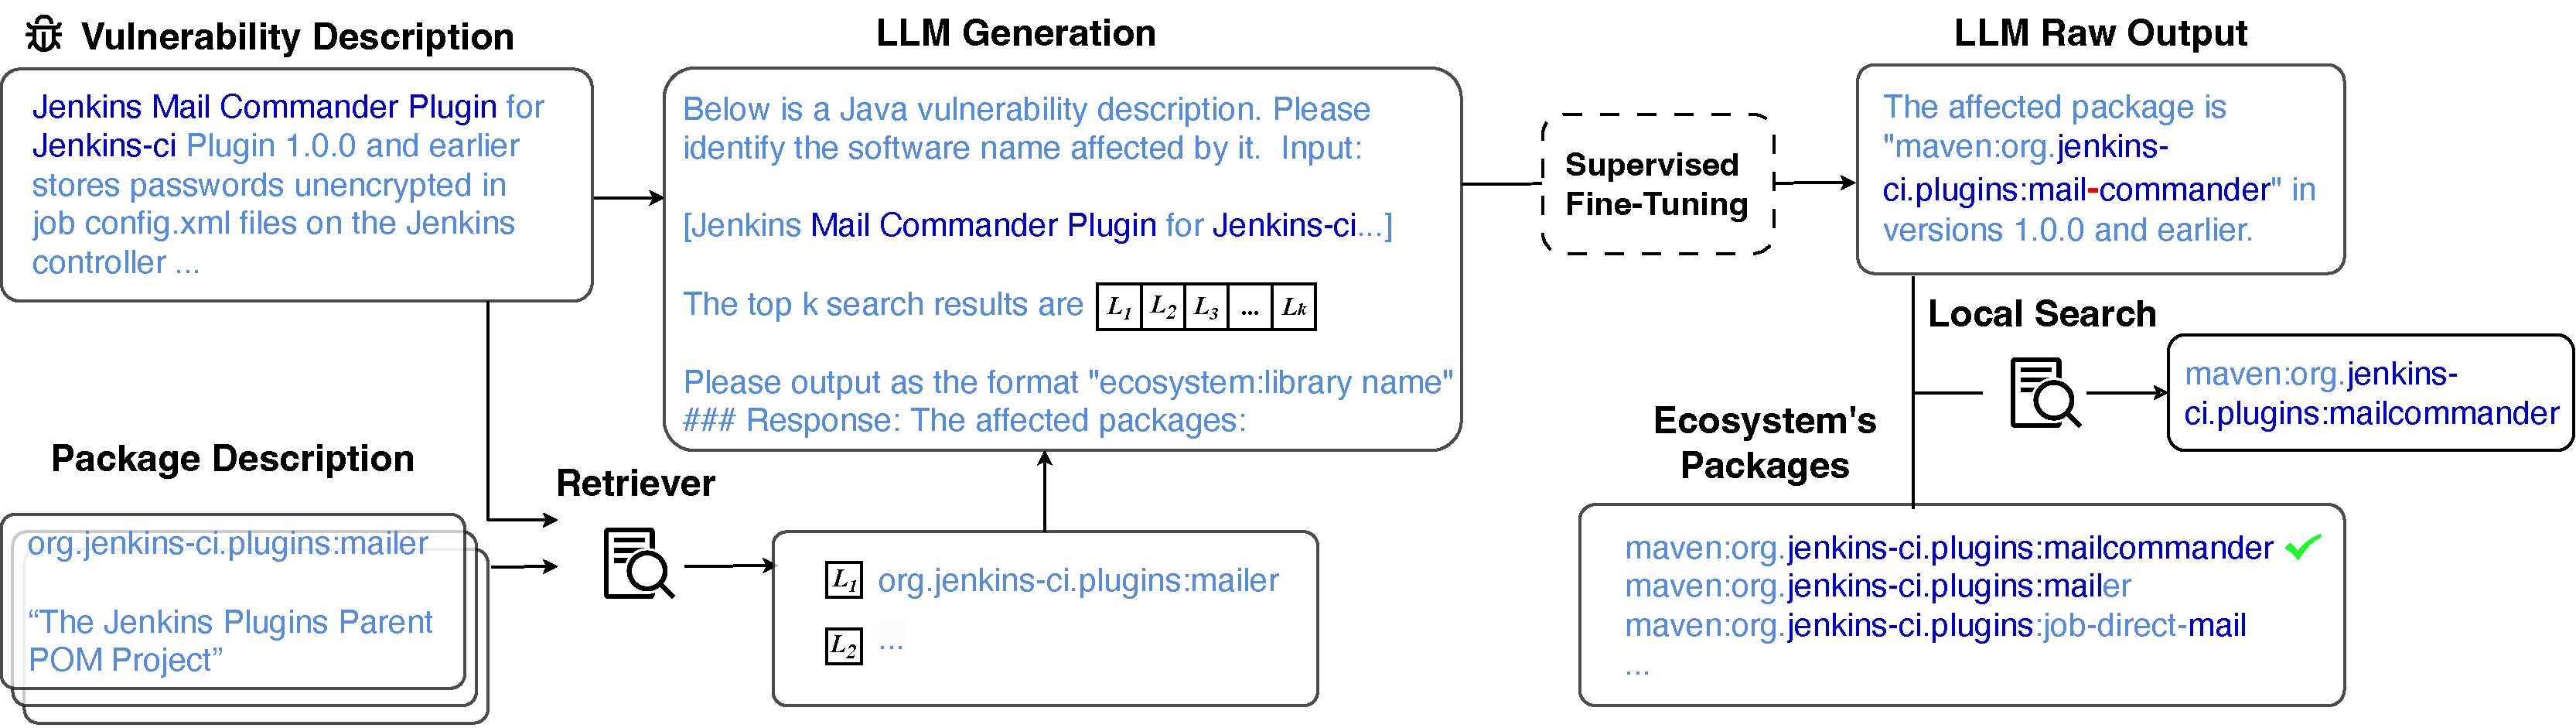
\includegraphics[width=1\linewidth]{figures/workflow-v3.drawio.pdf}
\caption{The \detector{} Framework}
\label{fig: framework}
\vspace{-0.3cm}
\end{figure*}

From the study result, we draw the conclusion that post-processing by matching is a promising approach to solve Challenge 2. This is because the majority errors are Type 2 errors, while post-processing is the most effective in helping with Type 2 errors. For example, for \href{https://github.com/advisories/GHSA-264w-xrr7-6qqg}{CVE-2020-2167}, ChatGPT generates \textcolor{Red}{org.jenkins-ci.plugins}:\textcolor{Blue}{openshift-pipeline}. While the \textcolor{Blue}{suffix} is correct, the \textcolor{Red}{prefix} and \textcolor{Blue}{suffix} never co-occur in any existing package name. We can fix this case by matching the prefix to the closest co-occured one. 
%The average edit distance between ChatGPT output and the ground truth in Type 2 cases is 76\%. 
By applying a naive edit-distance matching on the ChatGPT output, the accuracy is improved from 42\% to 51\%. 



%We start by querying ChatGPT with 2,789 Java vulnerability descriptions collected in a recent work~\cite{vullibminer}. ChatGPT outputs the correct package names (exactly matching) 42\% of the time. Next, we randomly sample 100 from the remaining incorrect ones and manually annotate the error reasons. Since all Java packages are in the format of [group id]:[artifact id], we classify the errors into the 4 classes in Table~\ref{tab: fault case study}. First, for the first two types (63\%), either the group ID or the artifact ID is correct, we thus further try matching the generation output with the closest package name (based on edit distance), and find that 34.9\% errors can be fixed. For example, the generation output for \href{https://github.com/advisories/GHSA-264w-xrr7-6qqg}{CVE-2020-2167} contains the group id \CodeIn{com.openshift.jenkins} which does not exist. On the other hand, the closest package in the existing list is the correct one. Second, for the last two types of errors there exists a knowledge gap for ChatGPT to identify the correct package name.

%, e.g., ChatGPT fails to identify that DolphinScheduler refers to the package \CodeIn{org.apache.dolphinscheduler}. 
%From the pilot study result we conclude that: while the generative approach has a reasonable baseline accuracy, there exists room for potential improvement by matching the generation output with existing package names and enhancing the knowledge of the LLM. 


% \begin{table*}[t]
%     \centering
%     \caption{The Classified Reasons for ChatGPT's Incorrect Response in Maven}
%     \label{tab: fault case study}
% \scriptsize
% \begin{tabular}{lclll}
% \toprule
% \textbf{Fault Reason}                         & Number                    & Example                             & ChatGPT's Output                                                   & Ground Truth (Affected Packages)                                                         \\
% \midrule
% \textbf{Mixed Artifact ID}                    & 21                        & \href{https://github.com/advisories/GHSA-wv88-pf73-x22p}{CVE-2011-2730}                     & org.springframework:spring-framework                                    & org.springframework:spring-core                                      \\
% \multicolumn{5}{l}{\textit{Description:} ``VMware \textcolor{ForestGreen}{SpringSource Spring Framework} before 2.5.6.SEC03, $\dots$'', and ChatGPT mistakes token ``\textcolor{BrickRed}{framework}'' in its artifact ID.}                                                                                                                                                                                \\
% \midrule
% \textbf{Mixed Group ID}                       & 15                        & \href{https://github.com/advisories/GHSA-264w-xrr7-6qqg}{CVE-2020-2167}                       & org.jenkins-ci.plugins:openshift-pipeline                    & com.openshift.jenkins:openshift-pipeline                       \\
% \multicolumn{5}{l}{\textit{Description:} ``\textcolor{ForestGreen}{OpenShift Pipeline} Plugin 1.0.56 and earlier $\dots$'' without the group id, so ChatGPT uses a widely used one ``\textcolor{BrickRed}{org.jenkins-ci.plugins}''.}                                                                                                                                                                      \\
% \midrule
% \textbf{More/Fewer Tokens}                      & 28                        & \href{https://github.com/advisories/GHSA-3v63-f83x-37x4}{CVE-2015-1830}                       & org.apache.activemq:activemq                                 & org.apache.activemq:activemq-client                            \\
% \multicolumn{5}{l}{\textit{Description:} ``Directory traversal vulnerability $\dots$ in \textcolor{ForestGreen}{Apache ActiveMQ} 5.x before 5.11.2 $\dots$'', and ChatGPT lacks the token ``\textcolor{ForestGreen}{client}''.}                                                                                                                                                                                      \\
% \midrule
% \textbf{Misleaded Name}                       & 23                        & \href{https://github.com/advisories/GHSA-jpj4-5xwp-cv23}{CVE-2020-11974}                      & mysql:mysql-connector-java                                   & org.apache.dolphinscheduler:dolphinscheduler                   \\
% \multicolumn{5}{l}{\textit{Description:} ``In \textcolor{ForestGreen}{DolphinScheduler} 1.2.0 and 1.2.1, with \textcolor{BrickRed}{mysql} connector $\dots$'', and ChatGPT incorrectly captures ``\textcolor{BrickRed}{mysql}''.}                          \\
% \midrule
% \textbf{No Structural Output}                            & 13                        & \href{https://github.com/advisories/GHSA-fxp8-7h5w-h235}{CVE-2019-13234}                      & -                                                                  & org.opencms:opencms-core                                       \\
% \multicolumn{5}{l}{\textit{Description:} ``In the Alkacon \textcolor{ForestGreen}{OpenCms} Apollo Template 10.5.4 and 10.5.5 $dots$'', and ChatGPT repeats the unstructured description.}  \\
% \bottomrule
% \end{tabular}
% \end{table*}



% \noindent \textbf{A Generation Task:}

% \subsection{Challenges of Adopting LLMs}~\label{sec:empirical_study}

% Before employing LLMs to generate the names of affected libraries, we conduct an empirical study to investigate the challenges when directly querying LLMs.







% \subsubsection{Lack Sufficient Domain Knowledge}
% First, LLMs lack sufficient domain knowledge of these affected libraries.
% For example, in CVE-2022-24197, the affected library is \CodeIn{com.itextpdf:itext7-core} while its description only mentions the affected library's artifact ID \CodeIn{itext7-core}, and its group ID \CodeIn{com.itextpdf} is neglected. 
% This group ID can be complemented based on the domain knowledge that only \CodeIn{itext7-core} corresponds to only one group ID \CodeIn{com.itextpdf}.
% Second, LLMs might output incorrect (even non-existing) library names.



% \subsection{Our Motivation}


% \noindent \textbf{Model Inference:} For a set of unlabeled vulnerabilities $\mathcal{V}_{new}$, we use one learned mapping relationship, $\mathcal{M^{\prime}}$, to predict these vulnerabilities' affected libraries, $\mathcal{M^{\prime}} (\mathcal{V}_{new})$, which is a subset of all libraries $\mathcal{L}$.


% \subsection{Existing Approaches of Identifying Vulnerable Libraries}

% \textbf{LightXML:} LightXML~\cite{lightxml} is one representative XML approaches that identify vulnerable libraries. 
% It takes the input of a vulnerability's description and outputs the order of a set of candidate libraries.
% Specifically, LightXML represents vulnerability descriptions based on transformer-based models, e.g., BERT~\cite{bert} or RoBERTa~\cite{roberta}.
% Then it uses generative cooperative networks to score all label clusters divided by a balanced K-means~\cite{da2008structural} algorithm.
% In a recent study~\cite{lightxml}, LightXML is more effective and efficient than its preceding approaches, such as ExtremeText~\cite{wydmuch2018no}, Bonsai~\cite{khandagale2020bonsai} and FastXML~\cite{fastxml}.
% Now that LightXML takes only the library names as labels, it can only predict full-shot libraries, i.e., $\mathcal{L}_{train}$.


% \textbf{Chronos:} Chronos~\cite{chronos} is another representative XML approach.
% Similar to other XML approaches, it also takes the input of a vulnerability's description and outputs the order of a set of candidate libraries.
% Chronos represents vulnerability descriptions and library names by TF-IDF and uses one SOTA XML algorithm, ZestXML to determine possible vulnerable libraries.
% Although ZestXML can identify vulnerable libraries from a candidate library set with a little portion of zero-shot ones, e.g., $\mathcal{L}_{train} \cup \mathcal{L}_{test}$ (2,817 libraries)~\cite{chronos}, it also fails to identify zero-shot libraries from all Java libraries, $\mathcal{L}$ (310,844 libraries).


% \textbf{VulLibMiner:} VulLibMiner~\cite{vullibminer} is one representative entity-linking approach that identifies vulnerable libraries. 
% It takes the descriptions of a vulnerability and all libraries as inputs.
% VulLibMiner first uses a TF-IDF algorithm to filter out a subset of candidate libraries and uses a BERT-FNN network on each pair of <vulnerability, candidate library> to determine whether they are correlated.
% A recent study~\cite{vullibminer} shows that VulLibMiner is more effective than XML approaches, especially in identifying zero-shot libraries.
% Considering the large number of Java libraries (e.g., 310,844 in Maven) for comparison compared, the TF-IDF algorithm cannot be avoided, and yet causes false negatives (i.e., some vulnerable libraries are missed).


% \subsection{Large Pre-trained Language Models}
% Large Pre-trained Language Models (LLMs) mainly follow the Transformer~\cite{vaswani2017attention} structure with an encoder to encode a given input and a decoder to generate output sequences from the encoded representation.
% These LLMs include billions of parameters and are pre-trained on billions of language corpus on the internet.
% In recent years, LLMs, such as GPT-3/4~\cite{gpt3, openai2023gpt4}, LLaMa~\cite{llama}, and starcoder~\cite{starcoder}, have been widely applied in software engineering~\cite{chen2021evaluating, xia2022practical} and security~\cite{chan2023transformer, tony2023llmseceval} tasks.
% Additionally, LLMs can comprehend the descriptions of vulnerabilities, thus improving the effectiveness of downstream tasks, such as vulnerability type classification~\cite{liu2023not} and providing attack and defense guidance~\cite{abdeen2023smet}.


% Although LLMs perform well in comprehending vulnerability descriptions, they face the hallucination challenge~\cite{maynez2020faithfulness, shuster2021retrieval}, where LLMs generate plausible-looking results that are factually incorrect. 
% Specifically, they might mix up two similar entities (e.g., library names), or make errors where just one token is incorrect.
% A recent study~\cite{lee2023benefits} shows that even one of the largest LLM, GPT-4~\cite{openai2023gpt4} cannot avoid hallucinations.
% Considering the large number of Java library names, addressing hallucinations becomes one of the main challenges of identifying vulnerable libraries.

%
% \noindent \textbf{Zero-shot Library Identification:} The affected libraries of $\mathcal{V}_{new}$ might not occur in the training dataset due to the data imbalance of the large number of Java libraries (310,844) and the small number of affected Java libraries (2,811 and 985 in two recent work~\cite{fastxml, vullibminer}).
% Therefore, the model is required to identify unseen libraries during prediction, and this task is established in machine learning as zero-shot learning~\cite{wang2019survey}.

% If denote $\mathcal{L}_{train}$ and $\mathcal{L}_{test}$ as the vulnerable library sets of the training and testing set, zero-shot libraries are defined as libraries not occurred in the training set:
% \begin{equation}
%     \mathcal{L}_{zero} = \{l \in \mathcal{L}_{test} \mid l \not\in \mathcal{L}_{train}\} 
% \end{equation}

% Then, zero-shot vulnerabilities are vulnerabilities affecting only zero-shot libraries.
% We divide the testing set, $\mathcal{V}_{test}$, into two independent subsets, zero-shot vulnerabilities, $\mathcal{V}_{zero}$, and non-zero-shot (a.k.a, full-shot) vulnerabilities, $\mathcal{V}_{full}$. 
% \begin{equation}
%     \begin{aligned}
%         \mathcal{V}_{zero} &= \{ v \in \mathcal{V}_{test} \mid \mathcal{M} (v) \subseteq \mathcal{L}_{zero} \} \\
%         \mathcal{V}_{full} &= \{ v \in \mathcal{V}_{test} \mid \mathcal{M} (v) \not\subseteq \mathcal{L}_{zero} \} \\
%     \end{aligned}
% \end{equation}

% These two subsets can be used to evaluate the effectiveness of identifying zero-shot vulnerable libraries and full-shot ones.
